\section{Segment Partition Example}
\label{appendix:segment_partition_example}

\begin{figure}[ht]
\centering
\setlength{\fboxsep}{0pt} 
\setlength{\fboxrule}{1.5pt}
\fcolorbox{blue}{white}{ 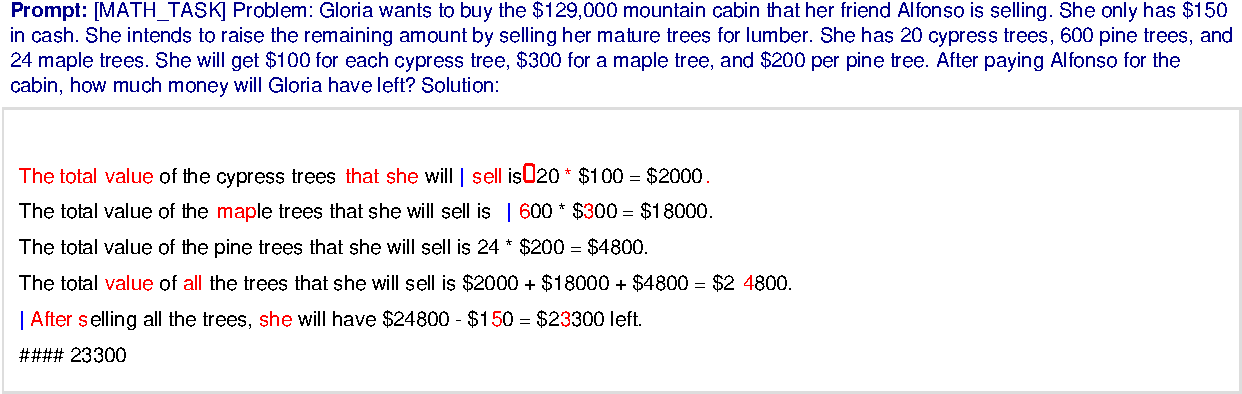
\includegraphics[width=0.98\textwidth]{figures/token_visualization_croped.pdf}}
  \caption{Segment partition based on fixed \emph{cutpoint} interval. Each row corresponds to a single step. Tokens marked in red indicate cutpoints (tokens with probability lower than 0.9). The blue vertical lines represent SPO segment boundaries.}
  \label{fig:segment_partition_cutpoint}
\end{figure}


Figure \ref{fig:segment_partition_cutpoint} shows a practical segment partition example. As we can see, many of the cutpoints (tokens whose probability is below a threshold) correspond to the places where the model makes mistakes. For instance, in the second step, the total value of the maple trees should be 24 * \$300, but the model outputs 600 * 300 and shows low confidence at the digit 6. If it had output 2 in this position, this step might have been correct. Similarly, in the final step, the calculation should be 24800 - 12900, but the model instead outputs 24800 - 150 and is uncertain at the digit 5. Had it produced a 2 at this point, the equation might have been correct. This case shows that cutpoints are the locations where the model’s reasoning trajectory can shift, and they are the main drivers behind “segment advantage”. Therefore, identifying and accurately assigning credit to these cutpoints is essential, which is consistent with our segment partition method (Section \ref{subsec:segment-partition-based-on-fixed-cutpoint-intervals}) and probability mask technique (Section \ref{subsec:policy-optimization-using-ppo-loss-with-prob-mask}). 

It is also worth noting that partitioning by line breaks, as in VinePPO, is not the most effective approach. For example, in step three, none of the tokens have probabilities below 0.9, indicating that the transition probabilities for all tokens in this step are very high. As a result, the estimated $V$ value at the beginning and end of this step will not differ significantly, thus the advantage for this segment will be close to zero. Allocating sampling budget to this step is likely to result in wasted samples.

Moreover, partitioning by step boundaries can lead to an uneven distribution of cutpoints, i.e., some segments may contain too many, while others include too few. Our goal in segment partition is to have each segment contain roughly the same number of potential ``turning points'', so that we can assign credit as efficiently as possible within a limited sampling budget. Step-based partition does not achieve this balance. This may help explain why our SPO-chain method can outperform VinePPO, even with fewer sampling points.